\documentclass[12pt]{article}
\usepackage[utf8]{inputenc}
\usepackage[spanish,es-lcroman, es-tabla]{babel}
\usepackage[autostyle,spanish=mexican]{csquotes}
\usepackage{amsmath}
\usepackage{amssymb}
\usepackage{nccmath}
\numberwithin{equation}{section}
\usepackage{amsthm}
\usepackage{graphicx}
\usepackage{epstopdf}
\DeclareGraphicsExtensions{.pdf,.png,.jpg,.eps}
\usepackage{color}
\usepackage{float}
\usepackage{multicol}
\usepackage{enumerate}
\usepackage[shortlabels]{enumitem}
\usepackage{anyfontsize}
\usepackage{anysize}
\usepackage{array}
\usepackage{multirow}
\usepackage{enumitem}
\usepackage{cancel}
\usepackage{tikz}
\usepackage{circuitikz}
\usepackage{tikz-3dplot}
\usetikzlibrary{babel}
\usetikzlibrary{shapes}
\usepackage{bm}
\usepackage{mathtools}
\usepackage{esvect}
\usepackage{hyperref}
\usepackage{relsize}
\usepackage{siunitx}
\usepackage{physics}
%\usepackage{biblatex}
\usepackage{standalone}
\usepackage{mathrsfs}
\usepackage{bigints}
\usepackage{bookmark}
\spanishdecimal{.}

\setlist[enumerate]{itemsep=0mm}

\renewcommand{\baselinestretch}{1.5}

\let\oldbibliography\thebibliography

\renewcommand{\thebibliography}[1]{\oldbibliography{#1}

\setlength{\itemsep}{0pt}}
%\marginsize{1.5cm}{1.5cm}{2cm}{2cm}


\newtheorem{defi}{{\it Definición}}[section]
\newtheorem{teo}{{\it Teorema}}[section]
\newtheorem{ejemplo}{{\it Ejemplo}}[section]
\newtheorem{propiedad}{{\it Propiedad}}[section]
\newtheorem{lema}{{\it Lema}}[section]

\marginsize{1.5cm}{1.5cm}{2cm}{2cm} 
\title{Coordenadas curvilíneas generales \\ {\large Matemáticas Avanzadas de la Física}}
\date{ }
\begin{document}
\renewcommand\labelenumii{\theenumi.{\arabic{enumii}}}
\maketitle
\fontsize{14}{14}\selectfont
\vspace{-2cm}
Con el fin de apoyar la construcción de un sistema de coordenadas curvilíneas generales, se muestra a continuación un par de figuras que serán de ayuda para elaborar en abstracto ese sistema general de referencia.
\par
Al asignar una serie de valores diferentes a $q_{k}$, generamos una familia de superficies en las que $q_{k}$ es constante. Si las funciones se han elegido correctamente, hay al menos una superficie que pertenece a cada una de las tres familias que pasa por cualquier punto arbitrario $P$ en el espacio. Por lo tanto, un punto en el espacio se caracteriza por la intersección de las tres superficies, $q_{1}$ = constante, $q_{2}$ = constante, $q_{3}$ = constante, llamadas \emph{superficies de coordenadas}. La superficie de coordenadas se llama para esa coordenada que es constante, las otras dos coordenadas son variables a lo largo de esa superficie.
\begin{figure}[H]
    \centering
    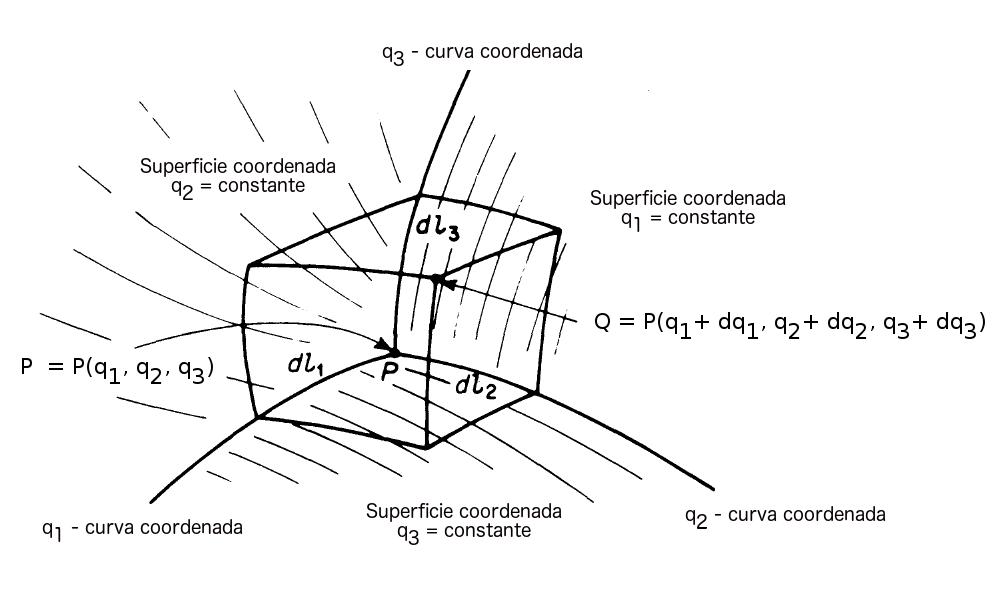
\includegraphics[scale=0.35]{Imagenes/CoordenadasCurvilineas_01.png}
    \caption{Sistema de coordenadas curvilíneas.}
\end{figure}
La intersección de dos superficies de coordenadas da como resultado una curva sesgada denominada \emph{curva de coordenadas}. Por ejemplo, la intersección de las superficies de coordenadas $q_{2}$ y $q_{3}$ da como resultado la curva de coordenadas etiquetada $q_{1}$.
\par
Como esta curva se encuentra simultáneamente en las superficies $q_{2}$ = constante y $q_{3}$ = constante, solo $q_{1}$ varía a medida que avanzamos a lo largo de la curva; de ahí, que se le llame curva de coordenada $q_{1}$.
\par
Tenemos que $\vu{i}_{1}$, $\vu{i}_{2}$ y $\vu{i}_{3}$ los vectores unitarios que son tangentes a las curvas de coordenadas $q_{1}$, $q_{2}$, $q_{3}$ respectivamente, en las direcciones en las que $q_{k}$ algebraicamente se incrementan.
\begin{figure}[H]
    \centering
    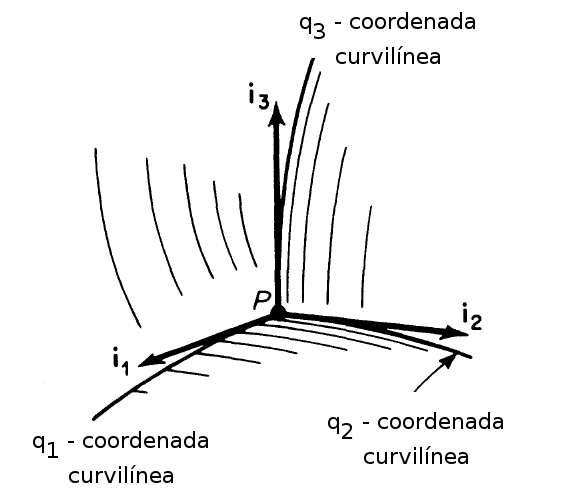
\includegraphics[scale=0.4]{Imagenes/CoordenadasCurvilineas_02.png}
    \caption{Vectores unitarios tangentes.}
\end{figure}
\end{document}